\clearpage
\begin{appendices}
\chapter{Appendix}

\section{Tabellen}

%% requirements tabelle
\begin{center}
	\begin{longtable}{|L{2.5cm}|L{3cm}|L{8.5cm}|}
		\caption[Liste der Requirements]{Auflistung der gesammelten Requirements der Smartwatch} \label{tab:table_requirements} \\
		\hline \multicolumn{1}{|c|}{\textbf{ID}} & \multicolumn{1}{c|}{\textbf{Name}} & \multicolumn{1}{c|}{\textbf{Text}} \\ \hline
		\endfirsthead

		\multicolumn{3}{c}%
		{{\bfseries \tablename\ \thetable{} -- Fortsetzung von vorheriger Seite}} \\
		\hline \multicolumn{1}{|c|}{\textbf{ID}} & \multicolumn{1}{c|}{\textbf{Name}} & \multicolumn{1}{c|}{\textbf{Text}} \\ \hline
		\endhead

		\hline \multicolumn{3}{|r|}{{Fortsetzung auf der nächsten Seite}} \\ \hline
		\endfoot

		\hline \hline
		\endlastfoot

		%% Ausgabe
		\multicolumn{3}{|l|}{\textbf{Ausgabe}} \\ \hline
		Ausgabe.01 & Displaygröße & Das Display soll eine Auflösung von 500x500 bei einer Bildschirmdiagonalen von 4 cm besitzen \\ \hline
		Ausgabe.02 & Farbdisplay & Das Display soll Farben darstellen können \\ \hline

		%% Usability
		\multicolumn{3}{|l|}{\textbf{Usability}} \\ \hline
		Usability.01 & Sichtbare Symbole &	Symbole sollten auf dem Display gut erkennbar sein \\ \hline
		Usability.02 & Touch-Symbolgröße &	Symbole, die eine Touch-Funktionalität besitzen, müssen mindestens 75\% des Bildschirms einnehmen \\ \hline

		%% Kapazität
		\multicolumn{3}{|l|}{\textbf{Kapazität}} \\ \hline
		Akku.01 & Akkulaufzeit & Eine Akkuladung soll bei normaler Benutzung mindestens 24 Stunden halten \\ \hline
		Akku.02 & Akkuladezeit & Der Akku soll innerhalb von 2 Stunden vollständig geladen werden \\ \hline
		Akku.03 & Akku: Induktionsladen & Der Akku soll über Induktion (z.B. Qi-Standard) geladen werden können \\ \hline

		%% Funktionen
		\multicolumn{3}{|l|}{\textbf{Funktionen}} \\ \hline
		Boot.01 & Bootvorgang maximal 10 Sekunden & Der Bootvorgang der Smartwatch soll maximal 10 Sekunden dauern \\ \hline
		Poweroff.01 & Ausschalten maximal 4 Sekunden & Das Ausschalten der Smartwatch soll maximal 4 Sekunden dauern \\ \hline
		Connection.01 &	Verbindung mit Smartphone & Das System soll sich mit einem Smartphone verbinden können \\ \hline
		Wasserdicht.01 & Wasserdicht bis 30 Meter & Das System soll Wasserdicht bis 30 Meter sein \\ \hline
		Notification.01 & Anzeigen der \glspl{Notification} & \glspl{Notification} sollen auf der Uhr angezeigt werden \\ \hline
		Notification.02 & \glspl{Notification} innerhalb einer Sekunde anzeigen & \glspl{Notification} sollen maximal nach einer Sekunde auf der Uhr angezeigt werden \\ \hline
		Connection.02 &	Verbindung mit Smartphone in 4 Sekunden & Die Verbindung mit dem Smartphone  muss in maximal 4 Sekunden hergestellt werden \\ \hline

		%% Ergonomie
		\multicolumn{3}{|l|}{\textbf{Ergonomie}} \\ \hline
		Ergonomie.01 & Auswechselbares Armband & Das Armband der Uhr soll ausgewechselt werden können \\ \hline
		Ergonomie.Gewicht.01 & Gesamtgewicht & Das Gesamtgewicht der Uhr soll maximal 50 Gramm wiegen \\ \hline

	\end{longtable}
\end{center}


\section{Diagramme}

\begin{figure}[h]
\centering\
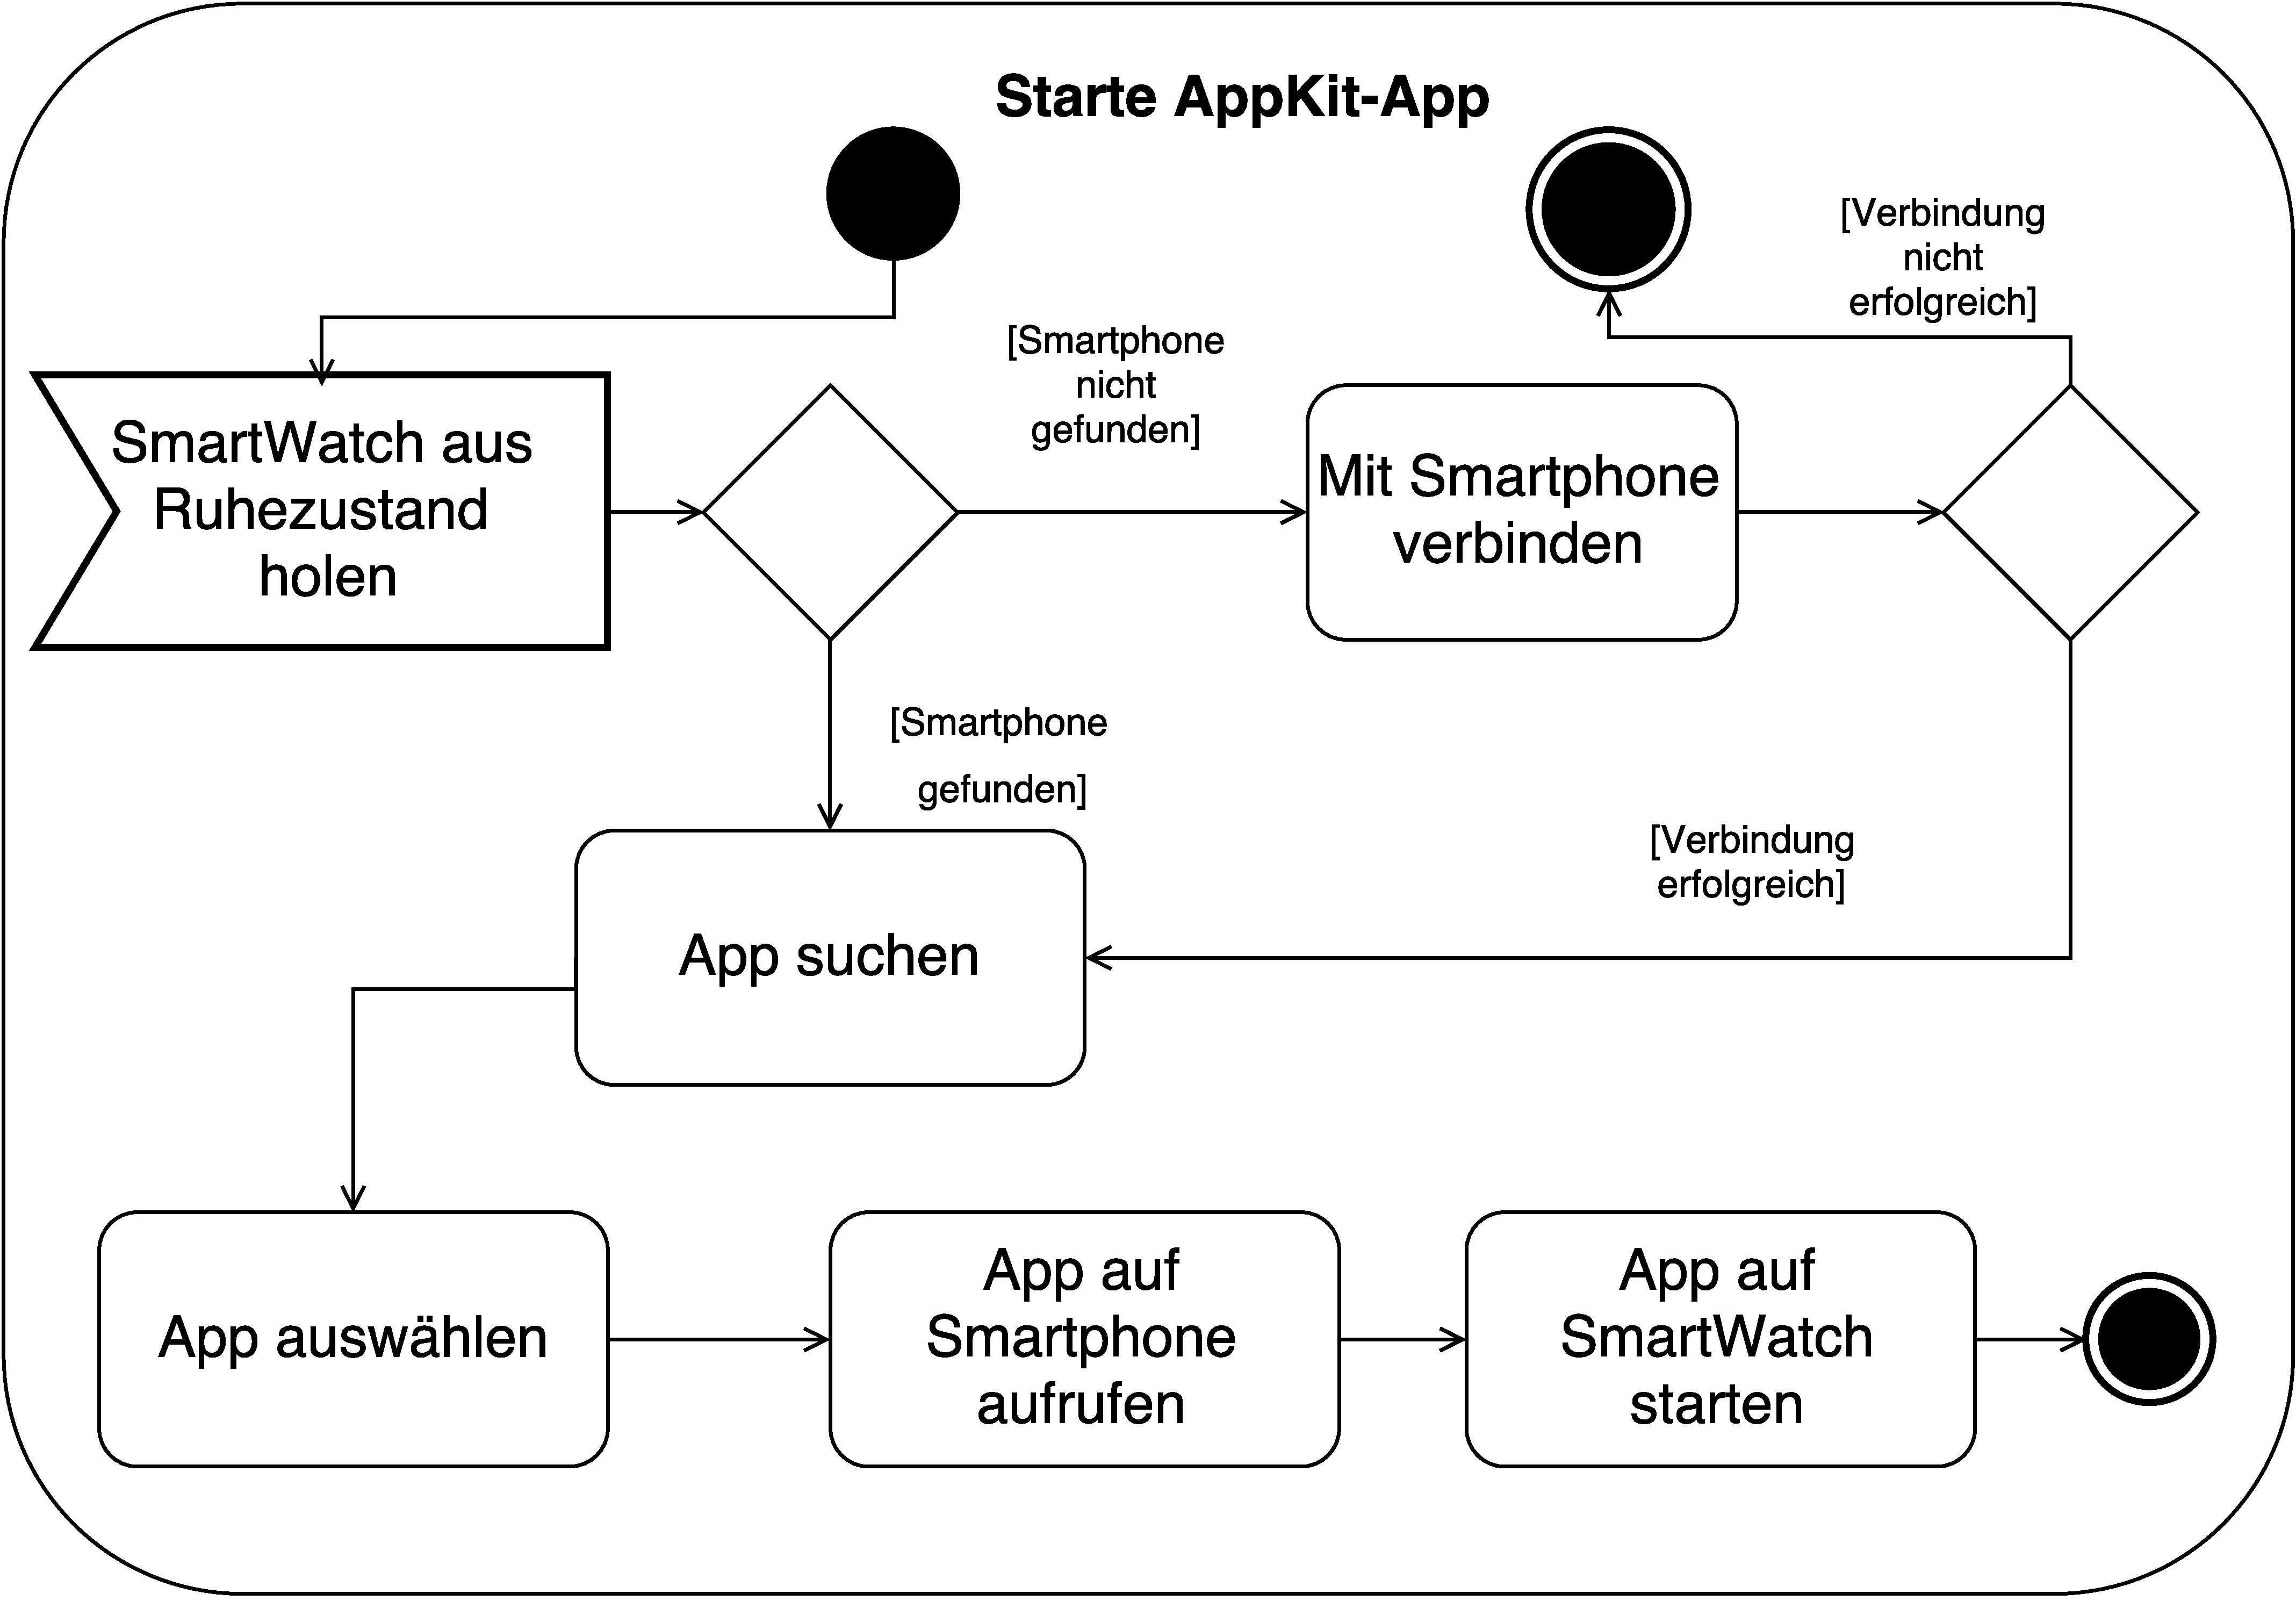
\includegraphics[width=\textwidth]{img/activityAppKit}
\caption{Starten einer AppKit-Applikation durch den Benutzer.}\label{fig:activityAppKit}
\end{figure}

\begin{figure}[h]
\centering\
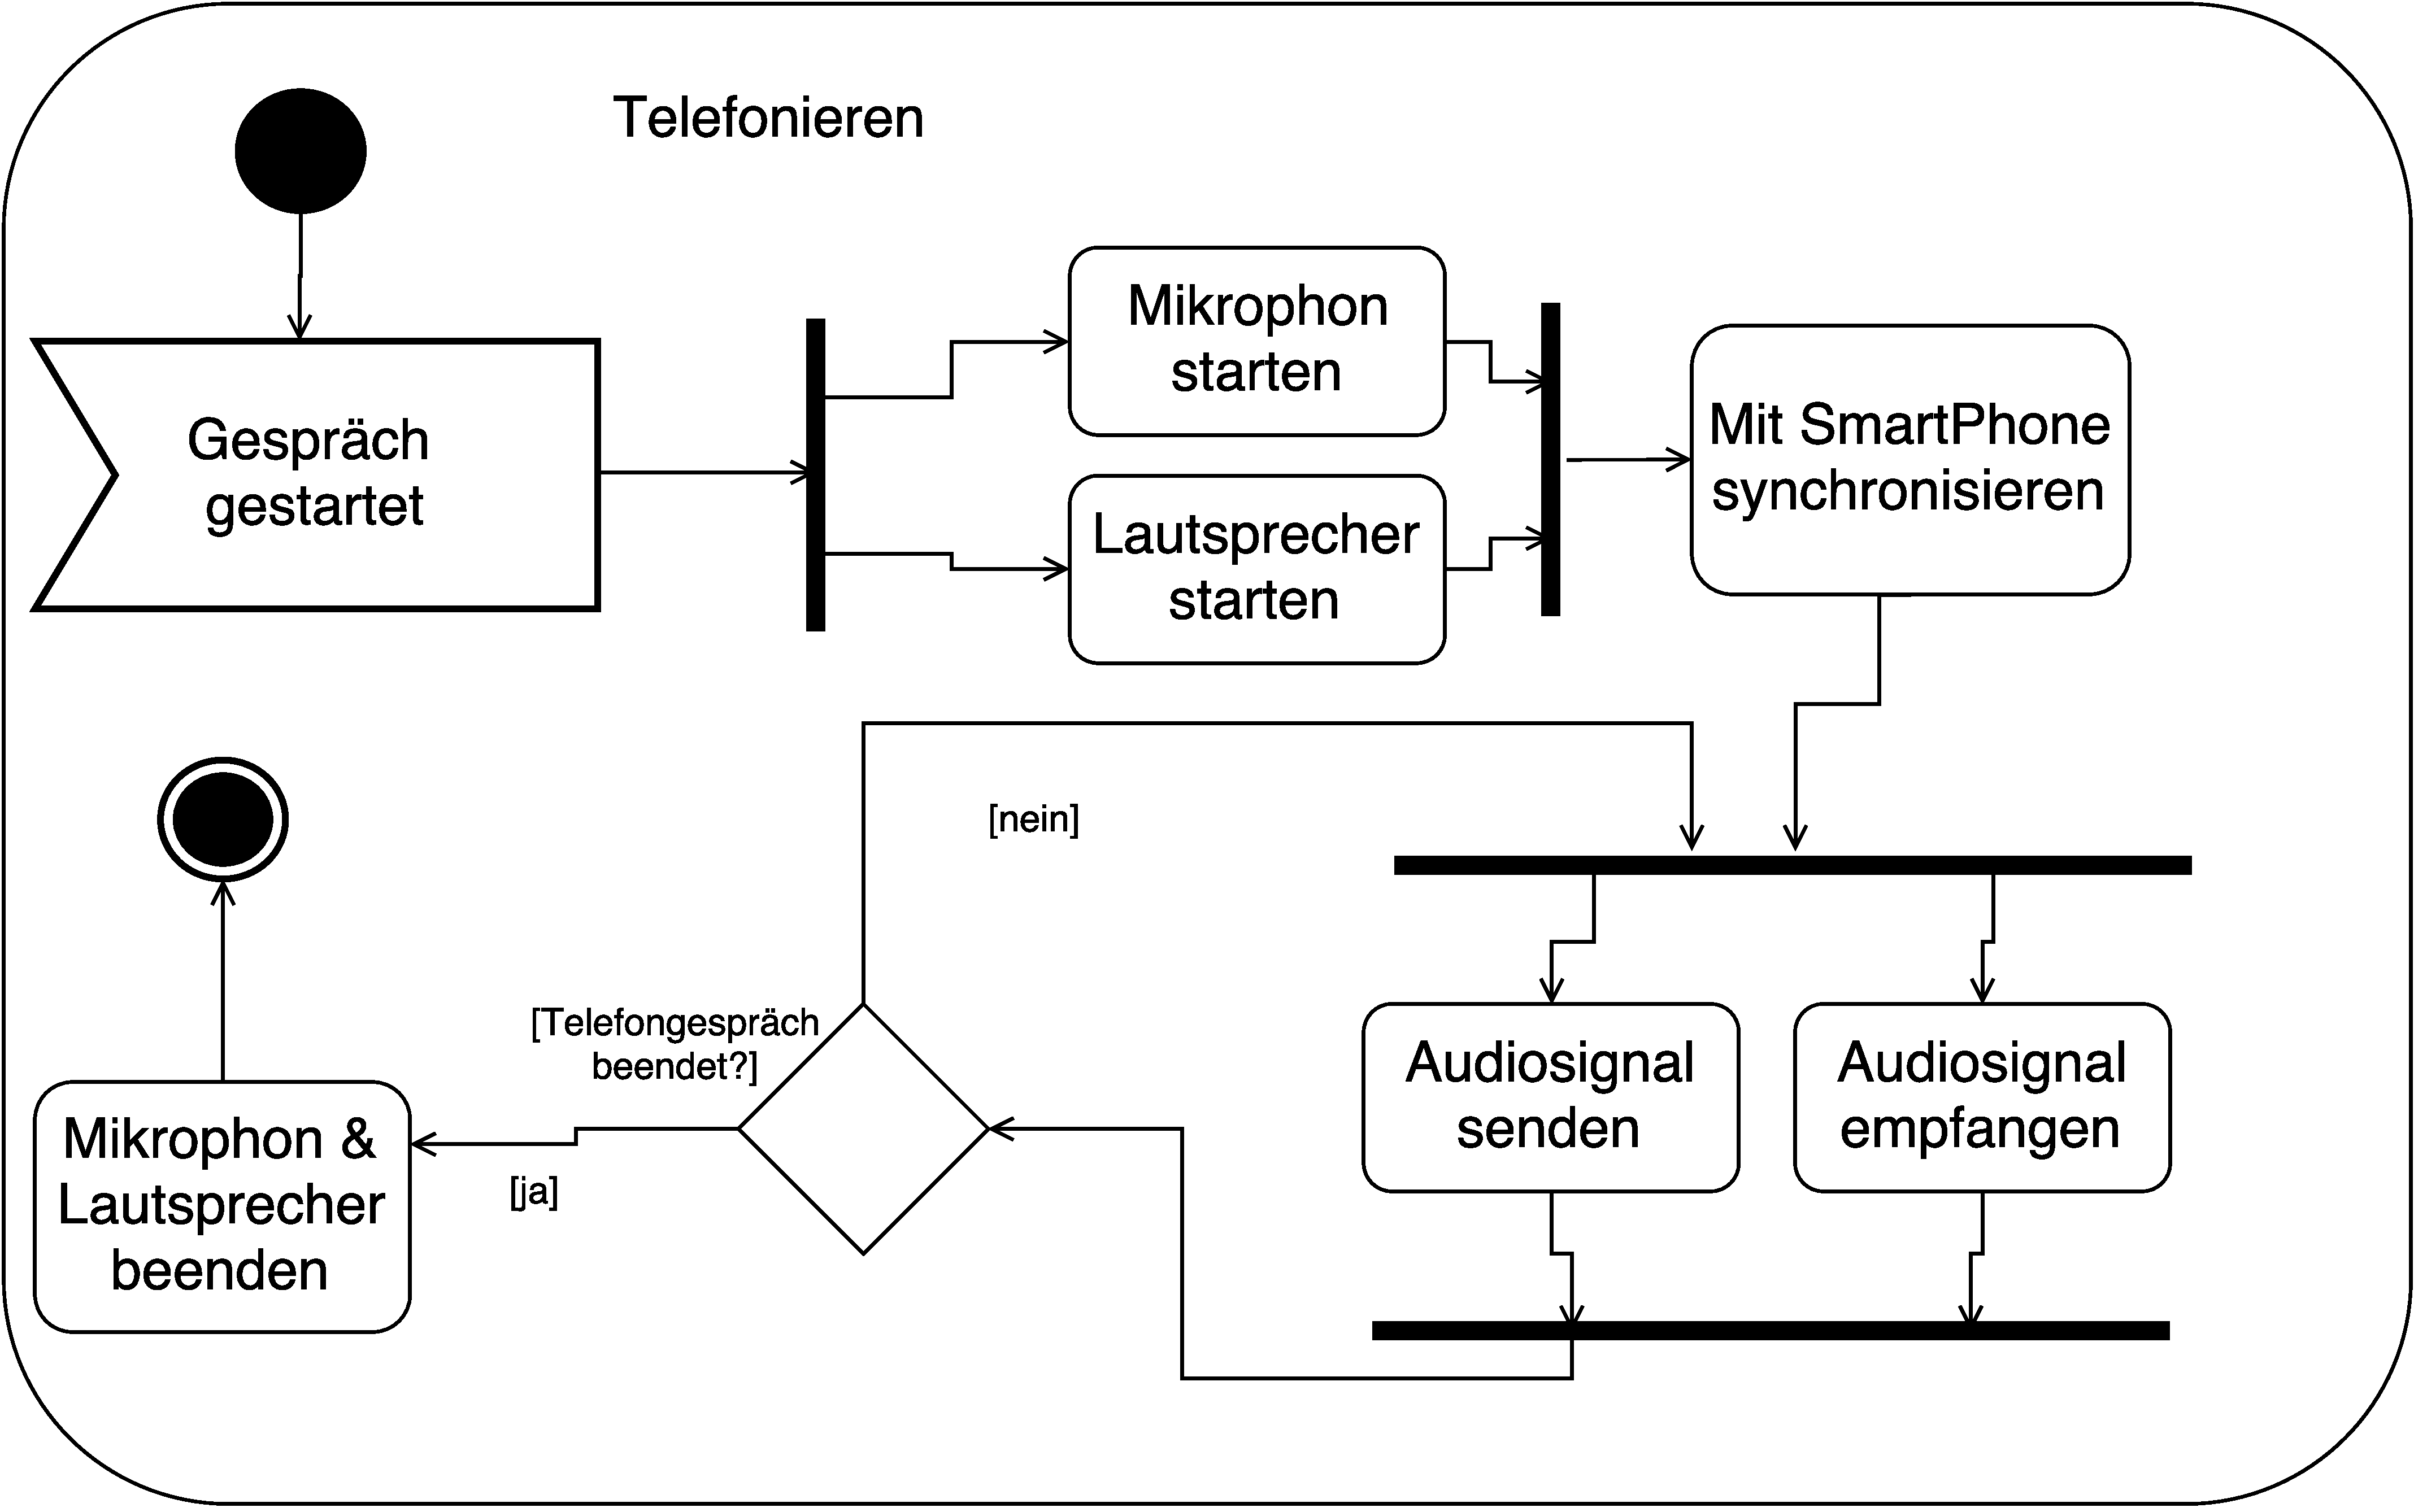
\includegraphics[width=\textwidth]{img/activityTelefonieren}
\caption{Verhalten der SmartWatch bei einem Telefonat.}\label{fig:activityTelefonieren}
\end{figure}

\begin{figure}[h]
\centering\
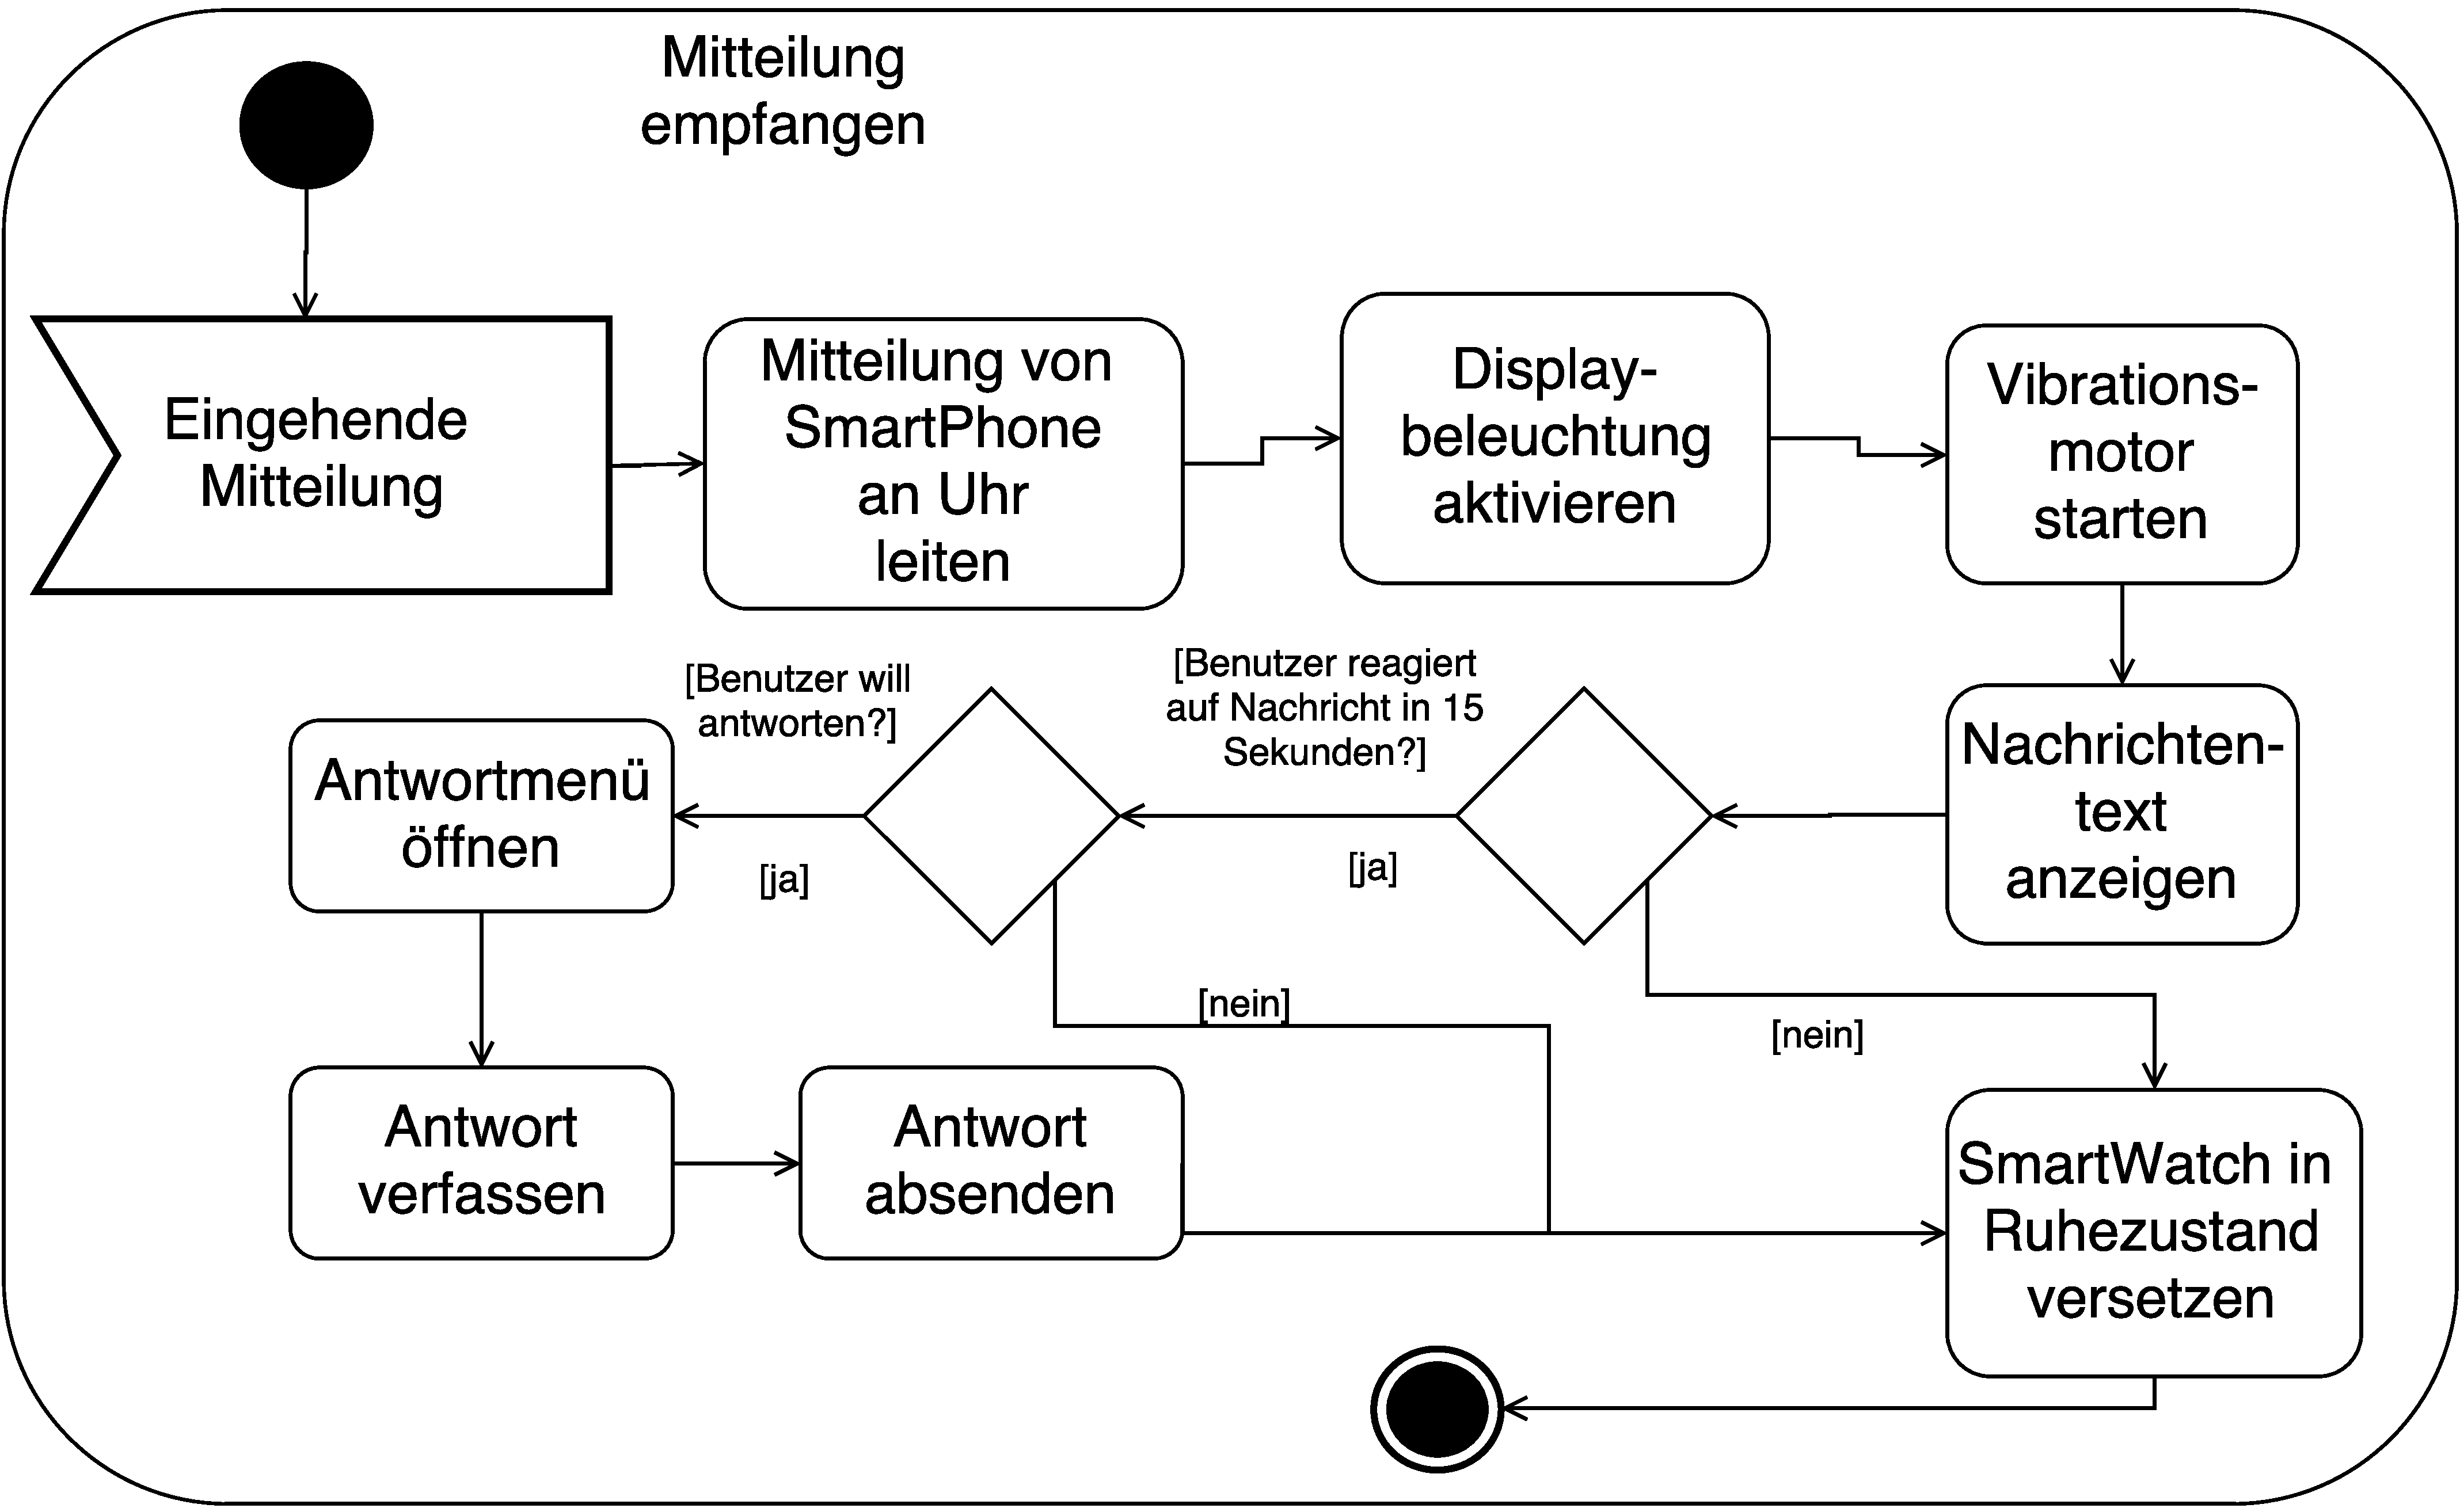
\includegraphics[width=\textwidth]{img/activityMitteilung}
\caption{Verhalten der SmartWatch bei einer eingehenden Mitteilung.}\label{fig:activityMitteilung}
\end{figure}

\section{Sonstiges}

\begin{figure}[h]
\centering\
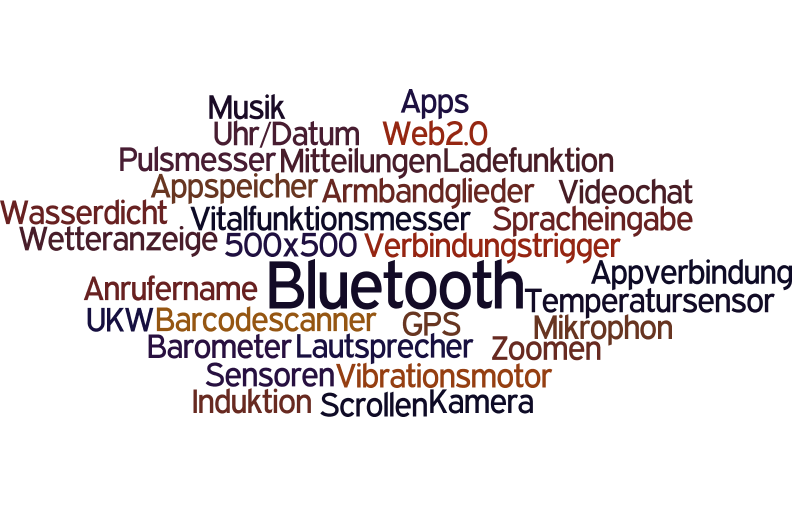
\includegraphics[width=\textwidth]{img/tagcloud}
\caption{Ideensammlung für die zu entwickelnde SmartWatch.}\label{fig:tagcloud}
\end{figure}

\end{appendices}
